\pdfoutput=1
\documentclass{article}
\usepackage{nips07submit_e}
\usepackage{amsmath}
\usepackage{graphicx}
\usepackage{algorithm2e}
\usepackage{times}
\usepackage{ifthen}

% ----------------------------------------------------------------
\vfuzz2pt % Don't report over-full v-boxes if over-edge is small
\hfuzz2pt % Don't report over-full h-boxes if over-edge is small

\newcommand{\OPT}{\textsf{OPT}}
\newcommand{\NULL}{\textsf{null}}

% ==============================================
% TEXT MANIPULATION MACROS, BASIC MACROS
% ==============================================
\newcommand{\ignore}[1]{}
\newcommand{\myskip}{\myvspace{-1mm}}
\newcommand{\captionsmall}[1]{\caption{\small #1}}
\newcommand{\commentout}[1]{}

\newcommand{\cf}{\emph{cf.}}
\def \etal {\emph{et al.}\ }

\newcommand{\ith}{\ensuremath{i^{\mathrm{th}}}\xspace}
\newcommand{\jth}{\ensuremath{j^{\mathrm{th}}}\xspace}
\newcommand{\tth}{\ensuremath{t^{\mathrm{th}}}\xspace}



% ==============================================
% REFERENCES
% ==============================================
\newcommand{\citet}[1]{\cite{#1}}
\newcommand{\citep}[1]{\cite{#1}}
\newcommand{\citecf}[1]{(\cf, \cite{#1})}

\newcommand{\tableref}[1]{Tab.~\ref{#1}}
\newcommand{\figref}[1]{Fig.~\ref{#1}}
\newcommand{\vfigref}[1]{Fig.~\vref{#1}}
\newcommand{\fullfigref}[1]{Fig.~\ref{#1} on page~\pageref{#1}}
\newcommand{\eqnref}[1]{Eq.~(\ref{#1})}
\newcommand{\secref}[1]{Sec.~\ref{#1}}
\newcommand{\thmref}[1]{Theorem~\ref{#1}}
\newcommand{\propref}[1]{Prop.~\ref{#1}}
\newcommand{\lemref}[1]{Lemma~\ref{#1}}
\newcommand{\corref}[1]{Corollary~\ref{#1}}
\newcommand{\algref}[1]{Alg.~\ref{#1}}
\newcommand{\lineref}[1]{Line~\ref{#1}}
\newcommand{\probref}[1]{Problem~(\ref{#1})}


% ==============================================
% LIST ENVIRONMENTS
% ==============================================

\newcommand{\denselist}{
    \itemsep -3pt\topsep-8pt\partopsep-8pt
}

\newcommand{\denselistbib}{
    \itemsep 0pt\topsep-4pt\partopsep-5pt
}

\newenvironment{Enum}{
\vspace{-0.5em}
\begin{enumerate}
   \setlength{\itemsep}{0.25em}%{3pt}
  \setlength{\parskip}{0em}
  \setlength{\parsep}{0em}}
{\end{enumerate}\vspace{-0.5em}}

\newcounter{myLISTctr}
\newcommand{\initOneLiners}{%
    \setlength{\itemsep}{0pt}
    \setlength{\parsep }{0pt}
    \setlength{\topsep }{0pt}
%      \usecounter{myLISTctr}
}
\newenvironment{OneLiners}[1][\ensuremath{\bullet}]
    {\begin{list}
        {#1}
        {\initOneLiners}}
    {\end{list}}

% ==============================================
% COMMON SETS, OBJECTS, and VARIABLES
% ==============================================
\newcommand{\integers}{\ensuremath{\mathbb{Z}}}
\newcommand{\nats}{\ensuremath{\mathbb{N}}}
\newcommand{\reals}{\ensuremath{\mathbb{R}}}
\newcommand{\Real}{\mathbb R}
\newcommand{\NonNegativeReals}{\ensuremath{\mathbb{R}_{\ge 0}}}

\newcommand{\eps}{\varepsilon}
\newcommand{\distrib}{{\mathcal{D}}}
\newcommand{\family}{{\mathcal{F}}}

% complexity classes
\newcommand{\class} [1] {\textrm{#1}} % bf or sc or rm?
\renewcommand{\P} {\class{P}}
\newcommand{\NP} {\class{NP}}

% ===================================================
% COMMONLY USED OPERATORS, FUNCTIONS, PARENS, ARROWS
% ===================================================
\def \argmax {\mathop{\rm arg\,max}}
\def \argmin {\mathop{\rm arg\,min}}


\newcommand{\paren} [1] {\ensuremath{ \left( {#1} \right) }}
\newcommand{\curlyparen} [1] {\ensuremath{ \left\{ {#1} \right\} }}
\newcommand{\bigparen} [1] {\ensuremath{ \Big( {#1} \Big) }}
\newcommand{\set}[1]{\ensuremath{\left\{#1\right\}}}
\renewcommand{\Pr}[1]{\ensuremath{\mathbb{P}\left[#1\right] }}
\DeclareMathOperator{\pr}{Pr} 
\newcommand{\prob}[1]{\ensuremath{\mathbf{Pr}\left[#1\right] }}
\DeclareMathOperator{\dist}{Dist}
\DeclareMathOperator{\dom}{dom}

\newcommand{\norm}[1]{\left\Vert#1\right\Vert}
\newcommand{\abs}[1]{\left\vert#1\right\vert}

% Expectations
\newcommand{\expt}[1]{\mathbb{E}\left[#1\right]}
\newcommand{\E}[1]{\ensuremath{\mathbb{E}\left[#1\right] }}
\newcommand{\Eunder}[2]{\ensuremath{\mathbb{E}_{#1}\left[#2\right] }}
\newcommand{\Econd}[2]{\ensuremath{\mathbb{E}\left[  {#1} \ \middle| \ {#2}\right] }}  % conditional expectation

\DeclareMathOperator*{\Var}{Var}
%\newcommand{\abs}[1]{\ensuremath{\left|#1\right|}}
\newcommand{\size}[1]{\ensuremath{\left|#1\right|}}
\newcommand{\ceil}[1]{\ensuremath{\left\lceil#1\right\rceil}}
\newcommand{\floor}[1]{\ensuremath{\left\lfloor#1\right\rfloor}}
%\newcommand{\norm}[2]{\ensuremath{\Vert {#1} \Vert_{#2}}}
\newcommand{\tuple}[1]{\ensuremath{\langle #1 \rangle}}
\newcommand{\func}[3]{\ensuremath{#1 : #2 \rightarrow #3}}
\newcommand{\poly}{\operatorname{poly}}

\newcommand{\To}{\longrightarrow}

% ==============================================
% ASYMPTOTICS
% ==============================================
\newcommand{\littleO}[1]{\ensuremath{o\paren{#1}}}
\newcommand{\bigO}[1]{\ensuremath{O\paren{#1}}}
\newcommand{\bigTheta}[1]{\ensuremath{\Theta\paren{#1}}}
\newcommand{\bigOmega}[1]{\ensuremath{\Omega\paren{#1}}}

% ==============================================
% PSEUDOCODE (these require the package algorithm2e)
% ==============================================
 \SetKw {KwEach} {\hspace{-1mm}each}
\SetKw {KwForEach} {for each}
\SetKw {KwFrom} {from}
\SetKw {KwSet} {set}
\SetKw {KwReturn} {return}
\SetKw {KwIf} {if}
\SetKw {KwThen} {then}
% ==============================================
% MISCELLANEOUS
% ==============================================
\renewcommand{\paragraph}[1]{\vspace{3mm}\noindent{\bf #1.} }



% ========= Andreas' Macros  ========================
% ----------------------------------------------------------------
\vfuzz2pt % Don't report over-full v-boxes if over-edge is small
\hfuzz2pt % Don't report over-full h-boxes if over-edge is smallq
% THEOREMS -------------------------------------------------------
%\newtheorem{thm}{Theorem}%[section]
\newtheorem{lemma}{Lemma}
\newtheorem{theorem}{Theorem}
\newtheorem{cor}[theorem]{Corollary}
%\newtheorem{lem}[thm]{Lemma}
\newtheorem{prop}[theorem]{Proposition}
\newtheorem{problem}[theorem]{Problem}
\newtheorem{example}[theorem]{Example}
%\theoremstyle{definition}
\newtheorem{defn}[theorem]{Definition}
%\theoremstyle{remark}
%\newtheorem{rem}[thm]{Remark}
%\numberwithin{equation}{section}

%-------------------------------------------------------------
%                       subfigure
%-------------------------------------------------------------

%% enable subfigures
%\usepackage{subfigure}

%\newbox\subfigbox
%\makeatletter
%  \newenvironment{subfloat}
%    {\def\caption##1{\gdef\subcapsave{\relax##1}}%
%     \let\subcapsave\@empty
%     \setbox\subfigbox\hbox
%       \bgroup}
%      {\egroup
%     \subfigure[\subcapsave]{\box\subfigbox}}
%\makeatother


% ---------------


% MISC OTHER MATH STUFF ---------------------
\newcommand{\cA}{{\mathcal{A}}}
\newcommand{\cB}{{\mathcal{B}}}
\newcommand{\cC}{{\mathcal{C}}}
\newcommand{\cD}{{\mathcal{D}}}

\newcommand{\cI}{{\mathcal{I}}}

\newcommand{\cP}{{\mathcal{P}}}
\newcommand{\cR}{{\mathcal{R}}}
\newcommand{\cS}{{\mathcal{S}}}
\newcommand{\cT}{{\mathcal{T}}}
\newcommand{\cU}{{\mathcal{U}}}
\newcommand{\cV}{{\mathcal{V}}}
\newcommand{\cW}{{\mathcal{W}}}
\newcommand{\cX}{{\mathcal{X}}}

\newcommand{\balpha}{{\mathbf{\alpha}}}
\newcommand{\ba}{{\mathbf{a}}}
\newcommand{\bh}{{\mathbf{h}}}
\newcommand{\bs}{{\mathbf{s}}}
\newcommand{\bt}{{\mathbf{t}}}
\newcommand{\bu}{{\mathbf{u}}}
\newcommand{\bv}{{\mathbf{v}}}
\newcommand{\bw}{{\mathbf{w}}}
\newcommand{\bx}{{\mathbf{x}}}
\newcommand{\by}{{\mathbf{y}}}
\newcommand{\bz}{{\mathbf{z}}}
\newcommand{\bZ}{{\mathbf{Z}}}

\newcommand{\hF}{{\widehat{F}}}
\newcommand{\sF}{\mathcal{\bar{F}}}
\newcommand{\bF}{{\overline{F}}}

\DeclareMathOperator{\kernel}{\mathcal{K}}
\DeclareMathOperator{\meanf}{\mathcal{M}}





\title{Infinitely-Armed Bandit Algorithms}

\author{
Matthew Faulkner\\
\\
\And
Jon Krause \\
\\
\And
Daniel Rosenberg \\
\\
}

% The \author macro works with any number of authors. There are two commands
% used to separate the names and addresses of multiple authors: \And and \AND.
%
% Using \And between authors leaves it to \LaTeX{} to determine where to break
% the lines. Using \AND forces a linebreak at that point. So, if \LaTeX{}
% puts 3 of 4 authors names on the first line, and the last on the second
% line, try using \AND instead of \And before the third author name.

\begin{document}

\maketitle

Here we consider an extension of the K-armed bandit problem to bandits with
an infinite number of arms.  In particular, we look at the Hierarchical
Optimistic Optimization ($\mathcal{X}$-armed)\cite{xarms08}
and Zooming \cite{kleinberg2008multi} algorithms, and
compare their behavior to that of a number of algorithms which merely
discretize the domain and run a standard finite-armed bandit algorithm.

\section{Introduction}

This is the introduction, where I cite a bunch of
things. \cite{auer2002finite} \cite{xarms08} \cite{kleinberg2008multi}
\cite{auer1995gambling} \cite{pandey2007multi}.

\section{Algorithms}
%%%%%%%%%%%%%%%%%%%%%%%%%%%%%%%%%%%%%%%%%%%%%%%%%%%%%%%%%%%%%%%%%%%%%%%%%%%%%

\subsection{Hierarchical Optimistic Optimization Algorithm}
% introduction and summary
% description of covering tree
% summarized pseudo code of the HOO algorithm
% discussion of regret bounds
% implementation notes.

The Hierarchical Optimistic Optimization (HOO) algorithm is a
no-regret algorithm for the case when the ``arms'' form a generic
measurable space $\cX$, and when each arm $x \in \cX$ is associated
with a fixed distribution $f(x)$ of rewards with finite support. Much
like the UCB algorithm, the HOO algorithm seeks to accurately estimate
the reward function where it has high value, while loosely estimating
the reward function where it has low value. This is accomplished by
incrementally building a covering of the space $\cX$ with fine
subdivisions where rewards are high, and coarse subdivisions
elsewhere. These coverings are maintained in a tree data structure
called a \emph{covering tree}. In the covering tree, the root covers
all of $\cX$; other nodes represent finer subsets of $\cX$. A
deterministic rule based on values stored at each node of the tree is
used to descend the tree until a leaf is reached. This leaf represents
a subset of $\cX$ from which to (arbitrarily) select the next arm. The
reward for that arm is used to update the values associated with all
nodes along the path from chosen leaf to root. The regret bounds of
the algorithm are in terms of a local smoothness property at the
maxima of the mean-reward function $f$.

\subsubsection{Covering Tree}\label{sss:coverTree}
The HOO algorithm requires an infinite binary tree where each node
represents a subset of $\cX$. We denote the $i^{th}$ node at level
$h$ as $(h,i)$, and its two children as $(h+1, 2i-1)$ and $(h+1,
2i)$. The subset of $\cX$ associated with node $(h,i)$ is denoted
as $\cP_{h,i}$.

The covering tree is required to satisfy two properties:
\begin{align*}
  \cP_{(1,0} &= \cX\\
  \cP_{h,i} &= \cP_{h+1,2i-1} \cup \cP_{h+1,2i}
\end{align*}

It is assumed that $\cX$ has a dissimilarity measure
$l(\cdot,\cdot)$. The diameter of a subset $A \subseteq \cX$ is
defined as $\sup_{x,y \in A}l(x,y)$. It is further assumed that there
are values $\rho < 1$, $\nu_1, \nu_2 > 0$ s.t. for all integers $h
\geq 0$ and $i = 1,2, \dots, 2^h$, the diameter of $\cP_{h,i}$ is at
most $\nu_1 \rho^h$ and that it contains an open ball of radius $\nu_2
\rho^h$. This assumption specifies that the volume of the subset
$\cP_{h,i}$ shrinks geometrically with the depth of node $(h,i)$.

\subsubsection{HOO Algorithm}
The HOO algorithm operates by maintaining a collection of subsets
which cover the space $\cX$, along with an upper bound of the expected
reward of points in each subset that holds in high probability. These
subsets are maintained in the covering tree. Each time an arm is
selected, a new and finer subset is added to the covering tree. Arms
are selected by optimistically ``zeroing in'' on regions of high
expected reward. In this way, the tree develops fine granularity
around subsets of $\cX$ with high expected reward, and coarse
granularity around subsets of $\cX$ with low expected reward.

%% The HOO algorithm works in two parts. First, to select an arm, a
%% downward pass is made through the covering tree until a leaf is
%% reached. An arm $x \in \cP_{leaf}$ is selected, and a reward is
%% received.. In the second part of the algorithm, an upward pass from
%% leaf to root is made. The values of all nodes along this path are u

\begin{algorithm}
  \SetKwData{Left}{left}\SetKwData{This}{this}\SetKwData{Up}{up}
  \SetKwFunction{Union}{Union}\SetKwFunction{FindCompress}{FindCompress}
  \SetKwInOut{Input}{input}\SetKwInOut{Output}{output}
  %initialization
  %$ \cT \leftarrow \{ (0,1) \}$\;
  %$B_{1,2} \leftarrow \infty$ \;
  %$B_{2,2} \leftarrow \infty$ \;
  \For{$i=1,2,\dots$}{
    leaf $\leftarrow$ descendToLeaf(root)\;
    %currentNode $\leftarrow$ root\;
    %% \While{currentNode has been instantiated}{
    %%   $B_{left} \leftarrow$ Bvalue(leftChild(currentNode))\;
    %%   $B_{right} \leftarrow$ Bvalue(rightChild(currentNode))\;
    %%   \uIf{$B_{left} > B_{right}$}{
    %%     currentNode $\leftarrow$ leftChild(currentNode)\;
    %%   }
    %%   \Else{
    %%     currentNode $\leftarrow$ rightChild(currentNode)\;
    %%   }
    %% }
    %instantiate currentNode\;
    %Choose arm $x$ in $\cP_{currentNode}$ and play it\;
    arm $\leftarrow$ chooseArm(leaf)\;
    $Y \leftarrow$ getReward(arm)\;
    %Choose arm $x$ in $\cP_{leaf}$ and play it\;
    %Receive reward $Y$\;
    %$\cT \leftarrow \cT \cup$ currentNode \;
    updateValues(leaf)\;
    %Update values on path from leaf to root\;
    %% \ForAll{$(h,i) \in$ pathToRoot(currentNode)}{
    %%   $T_{h,i} \leftarrow T_{h,i} + 1$\;
    %%   $\hat{\mu}_{h,i} \leftarrow (1 - \frac{1}{T_{h,i}})
    %%   \hat{\mu}_{h,i} + \frac{Y}{T_{h,i}}$\;
    %% }
    %% \ForAll{$(h,i) \in$ pathToRoot(currentNode)}{
    %%   $U_{h,i} \leftarrow \hat{\mu}_{h,i} + \sqrt{(2 \ln n) / T_{h,i}}
    %%   + \nu_1 \rho^{h}$\;
    %% }
    %$B_{H+1, 2I-1} \leftarrow \infty$\;
    %$B_{H+1, 2I} \leftarrow -\infty$\;
    %$\cT' \leftarrow \cT$\;
    %% \While{$\cT' \neq \{ (0,1) \}$}{
    %%   $(h,i) \leftarrow$ {\sc leaf}$(\cT')$\;
    %%   $B_{h,i} \leftarrow \min \{ U_{h,i}, \max B_{h+1,
    %%         2i-1},B_{h+1, 2i}  \}$ \;
    %%   $\cT' \leftarrow \cT' \setminus \{ (h,i) \} $ \;
    %% }
  }
  \caption{Hierarchical Optimistic Optimization}\label{alg:hooShort}
\end{algorithm}

%``Node selection works by comparing $B$-values and always choosing
%the node with the highest $B$-value.''

The following values are associated with each node $(h,i)$:
\begin{align*}
  N_{h,i}(n) &= \text{number of times node } (h,i) \text{ or its
    descendants was selected, up to time } n\\ 
  \hat{\mu}_{h,i}(n) &= \text{avg. reward received by } v_{h,i} \text{
    and its descendants up to time n.}\\
  U_{h,i}(n) &= \hat{\mu}_{h,i}(n) + \sqrt{\frac{2 \ln n}{N_{h,i}(n)}}
  + \nu_1 \rho^h\\
  B_{h,i}(n) &= \min\{ U_{h,i}(n), \max\{ B_{h+1,2i-1}, B_{h+1,2i}\} \}
\end{align*}

During the descent from root to leaf, the algorithm always descends to
the child of larger $B$ value, with ties broken arbitrarily. Nodes
which have not yet been added to the tree (i.e., the ``children'' of a
current leaf) are given a $B$-value of $\infty$. The operation
descendToLeaf returns a new leaf. An arm is drawn from
$\cP_{leaf}$. Once the reward $Y$ of this arm is received, the above
values $N$, $\hat{\mu}$, $U$, and $B$ are updated for all nodes
between the root and the new leaf.

Full pseudo-code is given in \algref{alg:hoo}.

\subsubsection{Regret Bounds}
The mean-payoff function $f$ is assumed to satisfy the condition that
$\forall \; x,y \in \cX$,
\begin{equation*}
  f^* - f(y) \leq f^* - f(x) + \max \{f^* - f(x), l(x,y) \}
\end{equation*}
for some dissimilarity function $l(\cdot, \cdot)$. Such a function is
called \emph{weakly Lipschitz}. Note that this amounts to requiring
(one-sided) Lipschitzness at the maxima, while only requiring a looser
condition at other points. The further a point is from the maxima, the
looser is the requirement on smoothness.

The expected regret of the HOO algorithm is bounded, up to a
logarithmic factor, by $\sqrt{n}$. The rate of growth depends on
the values $\nu_1$, $\nu_2$, and $\rho$; specifically, the rate of
growth does not depend on the dimensionality of the space.

\subsubsection{Implementation}
The primary component of the implementation is the cover tree. When
$\cX$ is an n-dimensional rectangle in $\reals^n$, the covering tree
can be implemented as a binary tree in which each node represents a
rectangular region, and where the two children of each node are
defined by splitting their parent's region along some coordinate axis
(e.g., splitting the longest side). Incidentally, this is known as a
$kD$-tree data structure. While this is sufficient for such spaces as
the unit hypercube, it is also sufficient for several other spaces
which can be defined by points in a unit hypercube, such as an
n-dimensional sphere (in polar coordinates) or torus.


%%%%%%%%%%%%%%%%%%%%%%%%%%%%%%%%%%%%%%%%%%%%%%%%%%%%%%%%%%%%%%%%%%%%%
\subsection{Zooming Algorithm}
When the number of arms is infinite, additional assumptions are needed
about the relationship between the arms. For instance, arms that are
\emph{close} should produce similar results. The Zooming Algorithm is
defined to work in any example where the arms form a metric space. In
each phase, certain arms are chosen to be \emph{active}, and the
algorithm chooses which arm to play from these active arms.

The Zooming Algorithm is composed of multiple phases, each of which is
composed of $2^{i_{ph}}$ rounds, where $i_{ph}$ is the current phase
number. In a given round, you \emph{activate} an arm if that arm is
not covered by another arm. Each arm covers a radius defined by
$r_t(v):=\sqrt{8*i_{ph}/(2+n_t(v)))}$ where $v$ is the active arm, and
$n_t(v)$ is the number of times a given arm has been chosen at time
$t$. Each time an arm is played, its radius shrinks, and at the
beginning of each round, you \emph{activate} arms until you have a
complete covering using a \emph{covering oracle}. This oracle can
either return an uncovered arm, or state that there is no such
arm. After the space is covered, you play the arm with the optimal
index, defined as $I_t(v):=\mu_t(v)+2*r_t(v)$

\begin{figure}[!ht]
  \begin{center}
    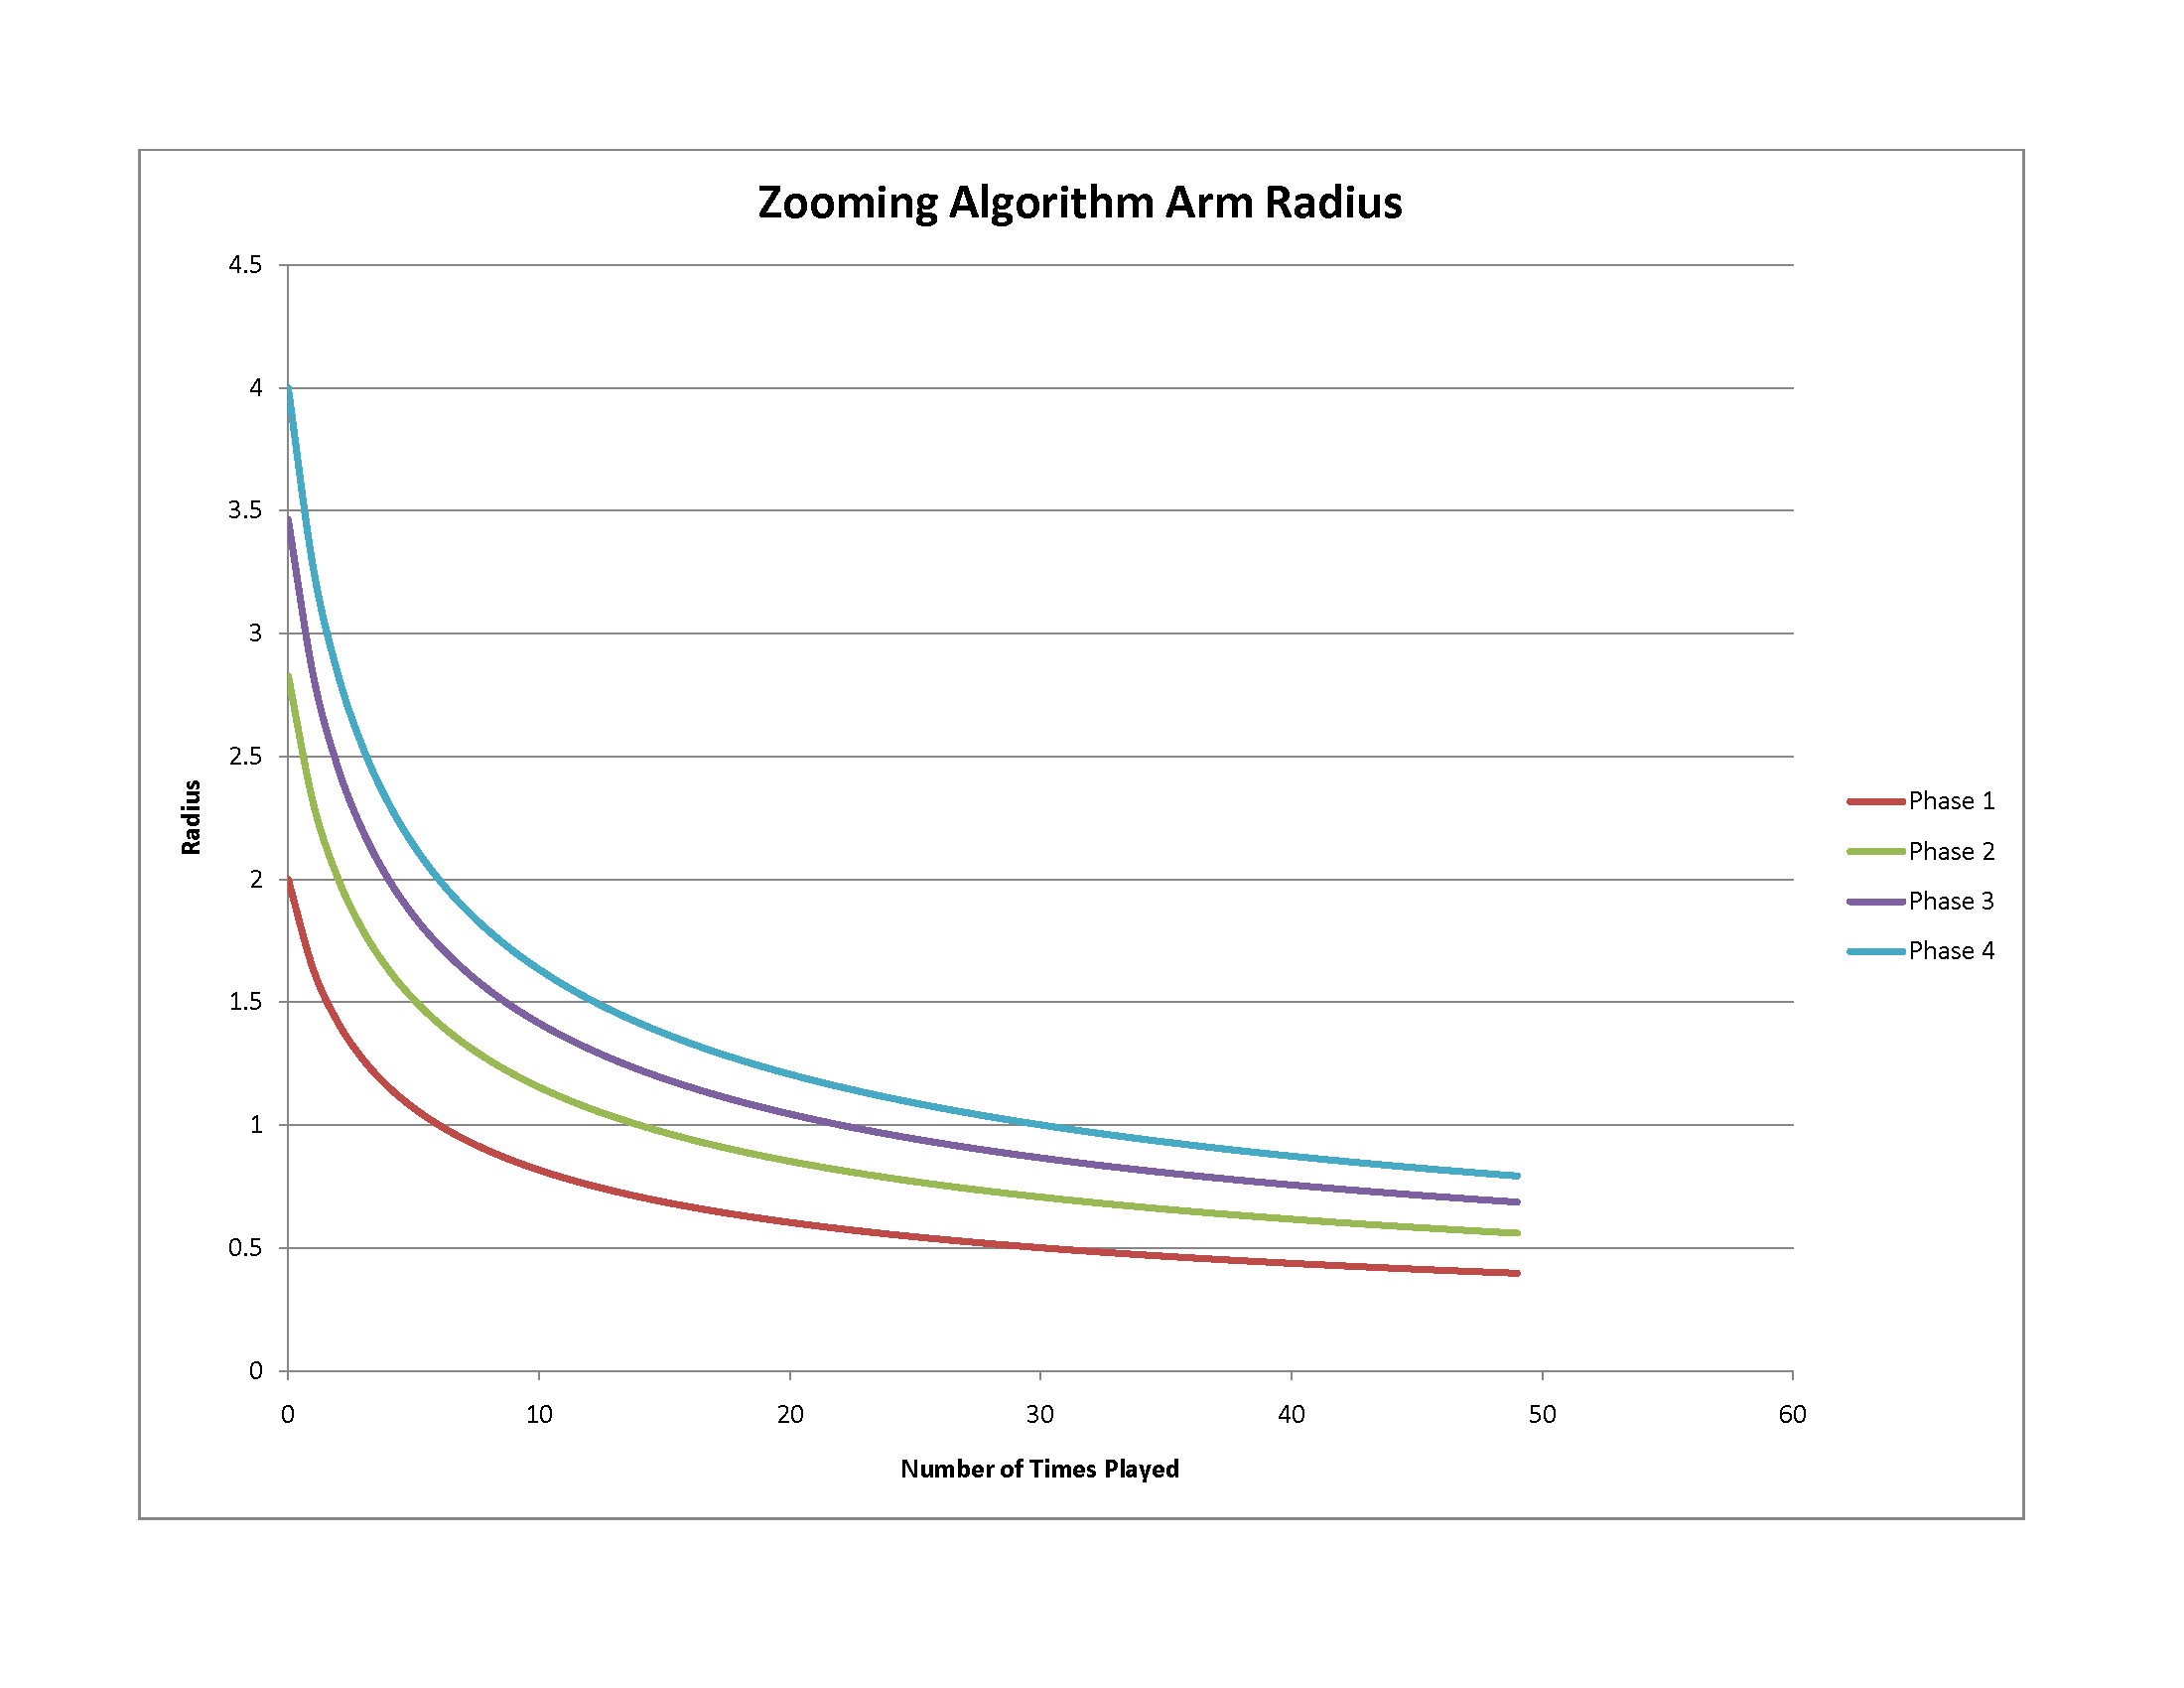
\includegraphics[width=5 in]{figures/ZoomingRadius.png}
     \caption{Arms cover less area the more they are played. The phase
       number only changes the scaling.}
     \label{fig:zoomradius}
  \end{center}
\end{figure}

Inbetween different phases, the Zooming Algorithm does not carry over
information. All that changes is $i_{ph}$. As $i_{ph}$ increases, the
index is effected increasingly more by how many times an arm has been
played. This means that earlier rounds have indices that are more
influenced by the $\mu_t(v)$, and will thus tend to exploit their
earlier finds more, while later rounds will perform more exploration
before zeroing in on the optimal arm. Given specific knowlege about
the problem at hand, this value could be optimized, allowing you to
run the zooming algorithm for a specific phase number.

\begin{figure}[!ht]
  \begin{center}
    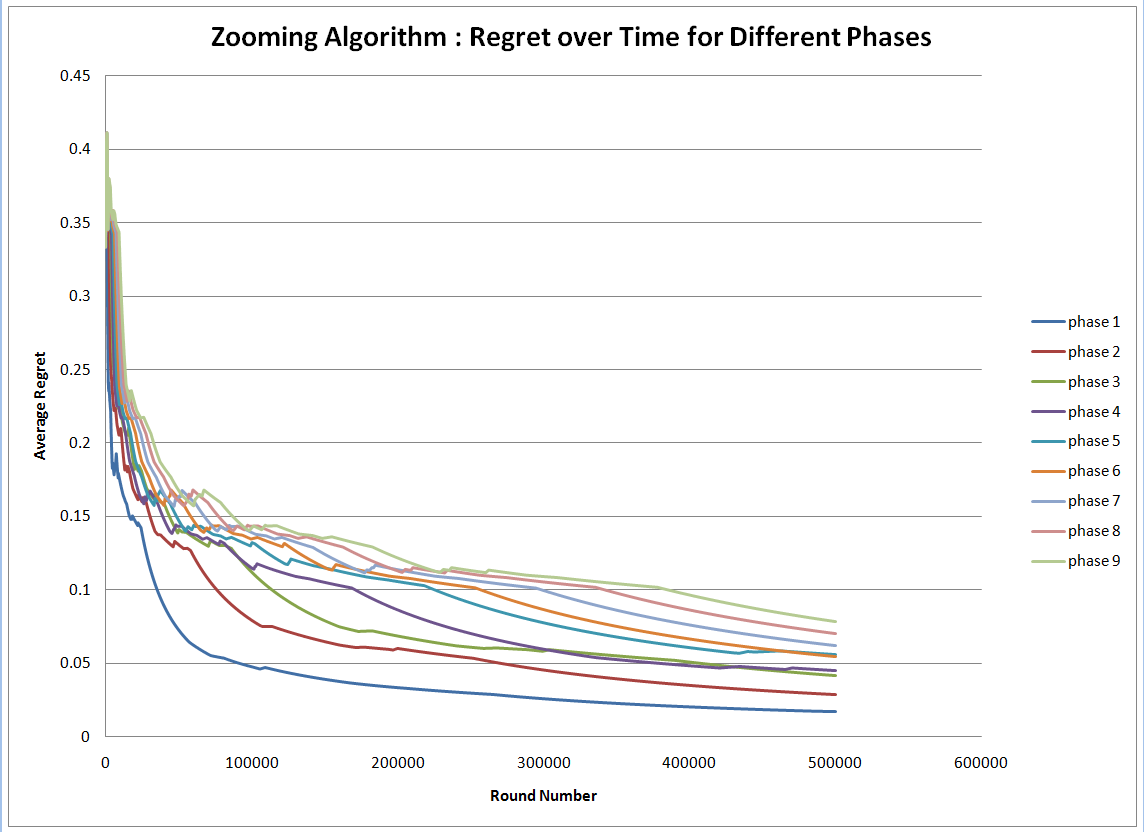
\includegraphics[width=5 in]{figures/Phase_Comparison.png}
     \caption{Here, the Zooming Algorithm was modified to run
       indefinitely on a specific phase number. As you can see, as a
       result of later phases doing more exploration, and having
       larger initial radii for their arms, later phases take longer
       to converge than earlier phases. The algorithm was run on a 2
       dimensional domain from 0 to 1 where reward is maximized at the
       point $(.3,.3)$. Reward was given by
       $\frac{1}{1+\mathrm{d}(v,(.3,.3))}$}
     \label{fig:zoomphase}
  \end{center}
\end{figure}



The runtime of the Zooming Algorithm depends very heavily on how the
covering oracle chosen behaves. This can be problematic, since the problem
is np-complete for the problem of hypercube coverings  \cite{Hoffmann05acovering} . In high dimensions,
the oracle can become quite expensive.

%%%%%%%%%%%%%%%%%%%%%%%%%%%%%%%%%%%%%%%%%%%%%%%%%%%%%%%%%%%%%%%%%%%%%%%%%%%%%
\subsection{Discretization Algorithms}
To test the $\mathcal{X}$-armed and Zooming algorithms, we have
implemented the $\epsilon$-greedy, UCB1 \cite{auer2002finite}, and
Exp3 \cite{auer1995gambling} finite-armed algorithms for the case
where whatever domain our bandit problem is over is discretized into
some finite number $K$ points.  In common to each algorithm is the
fact that the points are chosen randomly and uniformly from the
domain.  The intuition behind this choice is that, otherwise, it would
be relatively easy to construct a reward function that any
discretization would do terribly for, simply by ensuring that the
peaks of the reward function did not occur where the algorithm picked
a point.  For example, if arms were chosen in regular intervals from
the interval [0,1], i.e. at the points $\frac{i}{K+1}$, with $1 \leq i
\leq K$, then a reward function with a sharp peak at 0 would be
guaranteed to make any discretization algorithm perform poorly.
Choosing the arms at random at least guarantees that there is a chance
of doing well.  A brief description of the particulars of each
algorithm is now given.

\subsubsection{$\epsilon$-Greedy}
In round $t$, if $1 \leq t \leq K$ then play arm $t$.  Otherwise, play
randomly with probability $\epsilon$ and the arm with the best running
average otherwise.  We have implemented this algorithm using $\epsilon
= \frac{K}{t}$.

\subsubsection{UCB1}
In round $t$, if $1 \leq i \leq K$ then play arm $i$.  Otherwise, play
the arm that maximizes the quantity
\[
	\bar{r_i} + \sigma \sqrt{\frac{2 \log(t)}{p_i}}
\]
Where $\bar{r_i}$ is the average reward of arm $i$ so far, $p_i$ is the 
number of times arm $i$ has been played so far, and $\sigma$ is a parameter
that can be chosen to influence how much exploration is done.

\subsubsection{Exp3}
Initialize $w_i(1) = 1$ for all $1 \leq i \leq K$.  In round $t$, play
arm $i$ with probability
\[
	p_i(t) = \frac{\epsilon}{K} + (1 - \epsilon) \frac{w_i(t)}{\sum_j w_j(t)}
\]
With $i$ the arm that was played, update
\[
	w_i(t+1) = w_i(t)\gamma^{\frac{\epsilon r_i(t)}{K p_i(t)}}
\]
where $r_i(t)$ is the reward recieved, and set $w_j(t+1) = w_j(t)$ for all
other arms $j$.  $\gamma$ is a parameter that can be chosen to influence how
much exploration is done.  As in the $\epsilon$-greedy algorithm, we use
$\epsilon = \frac{K}{t}$.


% The analysis of the algorithms.  Basically going over each test case
% and what we can learn from them.

% Width of each figure.
\newcommand{\figwidth}{5in}

\section{Analysis}
Here we present an analysis of the test cases that we ran.  Unless
otherwise noted, $\sigma$ in the UCB1 algorithm is set to 1 and
$\gamma$ in the Exp3 algorithm is set to $e$.
% One-dimensional data
\subsection{One Dimension}
\subsubsection{Simple Reward Function}
As a very basic proof of concept, we ran the algorithms on the reward
function $r(x) = x$ over the unit interval [0,1].

\begin{figure}[!ht]
  \begin{center}
    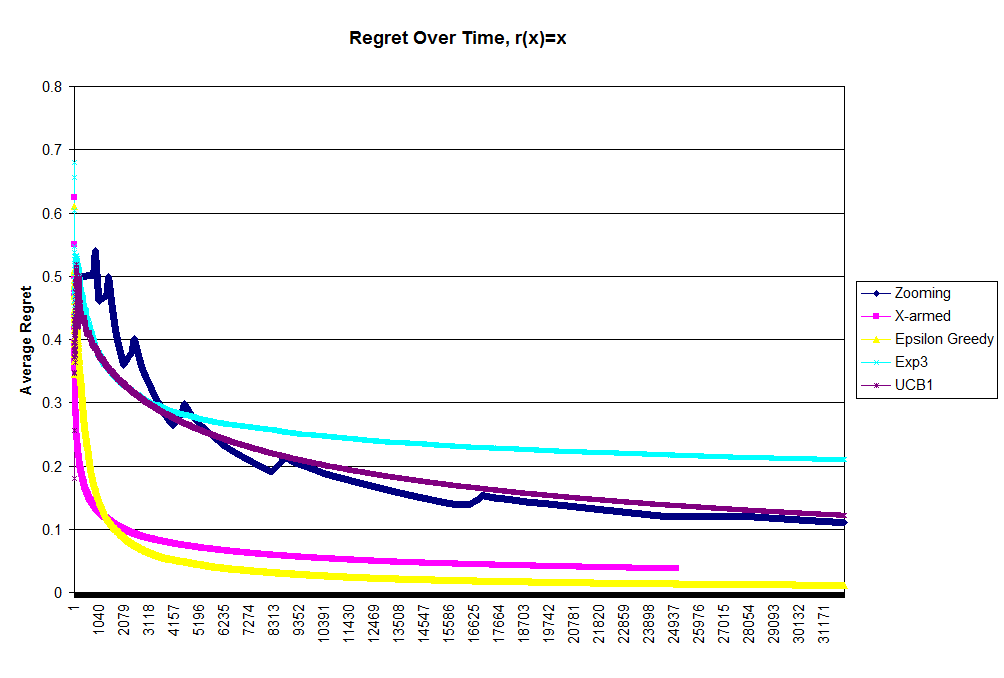
\includegraphics[width=\figwidth]{figures/1dsimpleplot.png}
     \caption{$r(x) = x$, 100 arms for discretization
     algorithms}
     \label{fig:1dsimple}
  \end{center}
\end{figure}

From figure \ref{fig:1dsimple}, we can see a number of facts.  First, at 
least in this case, the $\epsilon$-greedy algorithm is clearly the
best of all discretization algorithms, which is due to there being
no noise.  The $\mathcal{X}$-armed algorithm also does rather well,
but becomes expensive computationally as the number of rounds becomes
large due to having $O(n)$ time complexity in each round, where $t$ is
the number of rounds so far.  We can also see the characteristic bumps of
the Zooming algorithm, which are indicative of the fact that the Zooming
algorithm does not carry over information between phases.


\subsubsection{Noisy Reward Function}
Now we shall add some noise to our reward function.  The new reward
function is $r(x) = b(n_{0,1}(x))$, where $b(x) = 1$ with probability
$x$ and is 0 otherwise and $n_{\alpha_,\beta}(x)$ is $x$ times a random
number uniformly drawn from the interval $[\alpha, \beta]$.  The results
are presented in figure \ref{fig:1dnoise}

\begin{figure}[!ht]
  \begin{center}
    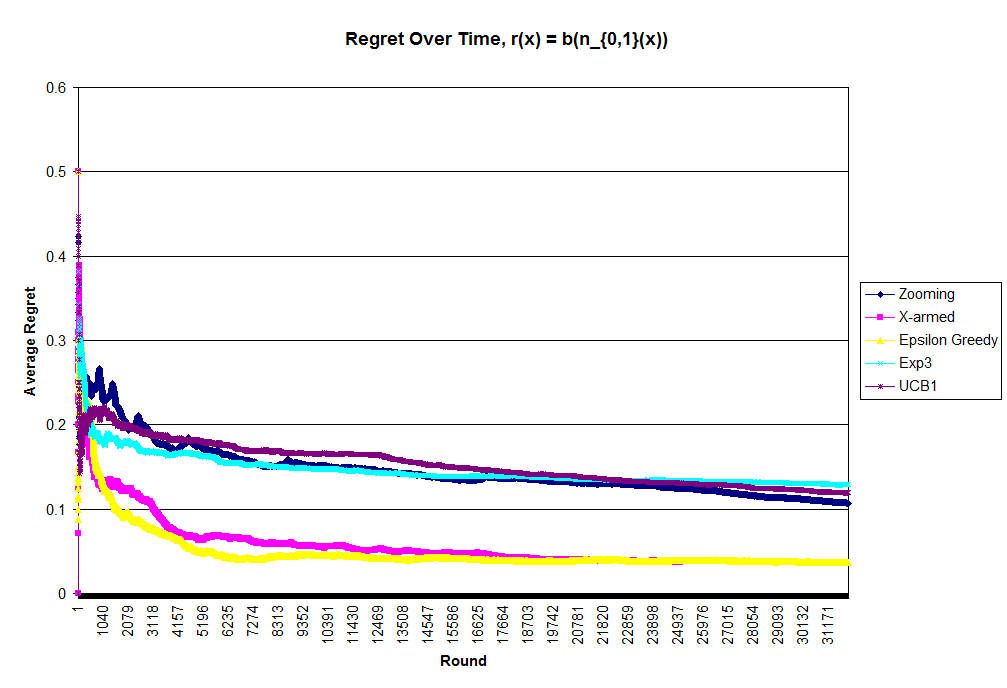
\includegraphics[width=\figwidth]{figures/1dnoiseplot.png}
     \caption{$r(x) = b(n_{0,1}(x))$, 100 arms for discretization
     algorithms}
     \label{fig:1dnoise}
  \end{center}
\end{figure}

For the most part, the algorithms perform basically as well as they did
in the no-noise case, with the notable exceptions that Exp3 algorithm did
better than before and the $\epsilon$-greedy algorithm did slightly worse
than before.  In the case of the $\epsilon$-greedy algorithm, this can be
partially attributed to the fact that the random discretization determines
how low the average regret can get, and that in this particular trial
the discretization was not very good.  We can tell that this is the true
reason for this behavior because otherwise, the $\epsilon$-greedy algorithm
would be converging more slowly, which does not appear to be the case.

Overall, from these simple 1D cases, we can see that
$\mathcal{X}$-armed algorithm appears to perform better than the Zooming
algorithm, although at the cost of being rather slow when the number of
rounds becomes large.  In a bandit setting, though, it is generally the
case that the reward function is somewhat costly to evaluate, and so the
computational cost of the $\mathcal{X}$-armed algorithm is not quite so
important.  Also, if we look at the very first few trials, the
$\mathcal{X}$-armed algorithm does fairly well rather quickly, whereas
the other algorithms take a little bit longer to fully explore the space.
For the discretization algorithms, though, this can be mitigated by
choosing a smaller number of arms to discretize the domain into.  In fact,
the very number of arms chosen for those algorithms is essentially a 
parameter helping to determine how much exploration to do -- more arms
will cause more exploration, and fewer arms will cause more exploitation.

\subsubsection{Prisoner's Dilemma - Changing Reward Function}
Here we present how the algorithms did against each other in an extension of
the Prisoner's Dilemma to a continuous-choice case.  As we shall have the
algorithms playing against each other, the reward function for a single
algorithm is not constant with respect to time, and so there is no reason to
suspect that the algorithms will still perform well, but it is an interesting
problem, even just to see the results.

First, we define our reward functions.  Given players 1 and 2, we define the
reward functions $r_1(x_1, x_2)$ and $r_2(x_1, x_2)$ by
\[
	r_1(x_1, x_2) = \frac{1}{3} x_1 - \frac{2}{3} x_2 + \frac{2}{3}
	r_2(x_1, x_2) = -\frac{2}{3} x_1 + \frac{1}{3} x_2 + \frac{2}{3}
\]
Note that each reward function is a plane, and that we have
\begin{gather*}
	(r_1(0,0), r_2(0,0)) = \left(\frac{2}{3}, \frac{2}{3}\right) \\
	(r_1(1,0), r_2(1,0)) = (1, 1) \\
	(r_1(0,1), r_2(0,1)) = (0, 1) \\
	(r_1(1,1), r_2(1,1)) = \left(\frac{1}{3}, \frac{1}{3}\right)
\end{gather*}
which is precisely the setup in a Prisoner's Dilemma game where 0 corresponds
to colluding and 1 corresponds to not colluding.

We use 100 arms for the discretization algorithms here, and each trial is run
through 5000 rounds.  We also introduce a modified $\mathcal{X}$-armed
algorithm which does a random walk down its covering tree with probability .1,
in the hopes that this will allow it to adapt to a changing reward function.
Here we present the average rewards over those rounds, where the first element
in a pair of numbers corresponds to the average reward for the row algorithm
and the second number corresponds to the average reward for the column
algorithm.  

\begin{tabular}{|c|c|c|c|c|c|c|}
\hline
& $\epsilon$-greedy & UCB1 & Exp3 & $\mathcal{X}$-armed &
Modified $\mathcal{X}$-armed & Zooming \\ \hline
$\epsilon$-greedy & .44, .39 & .60, .25 & .55, .27 & .47, .31 & .49, .35 &
.58, .25\\ \hline
UCB1 & & .48, .46 & .48, .46 & .37, .52 & .37, .49  & .46, .48 \\ \hline
Exp3 & & & .47, .44 & .36, .52 & .39, .46 & .48, .44 \\ \hline
$\mathcal{X}$-armed & & & & .59, .59 & .48, .49 & .53, .34 \\ \hline
Modified $\mathcal{X}$-armed & & & & & .50, .50 & .52, .35 \\ \hline
Zooming & & & & & & .53, .53 \\ \hline
\end{tabular}

As a sidenote, the algorithms that tended to do too much exploring in the
simple case of $r(x)=x$ tended to have the least convergence to an arm.
On the other hand, the $\epsilon$-greedy algorithm was relatively
convergent, almost always to relatively high values, which corresponds to
not colluding in the game and is the dominant strategy.  Also, the
deterministic algorithms, when run against themselves, obviously performed
identically to one another.  In particular, this causes the
$\mathcal{X}$-armed algorithm to always think that colluding is better, and
hence that matchup has the highest average rewards.
Now we shall examine the numbers.

Roughly speaking, the algorithms performed just about in the same order of
their performance on the simple $r(x)=x$ case.  This is somewhat surprising,
given that this reward function is not only slightly more complicated, but
changing over time.  In particular, the $\epsilon$-greedy algorithm was
just about always the best algorithm, the $\mathcal{X}$-armed algorithms
performed about the same, despite the modification, and the UCB1, Exp3,
and Zooming algorithms were all about the same.  Looking at the 5000
round mark in Figure \ref{fig:1dsimple}, this is an exact correlation, and
thus provides evidence for the hypothesis that the simple test cases
considered probably generalize in roughly a similar fashion, given how
different the reward function in this case was.


% ----------------------------------------------------------------
%\newpage
\bibliographystyle{plain}
{%\fontsize{9}{9}
\bibliography{report}
}

\end{document}